\begin{figure}[t!]
\vskip 0.05in
\begin{center}
\centerline{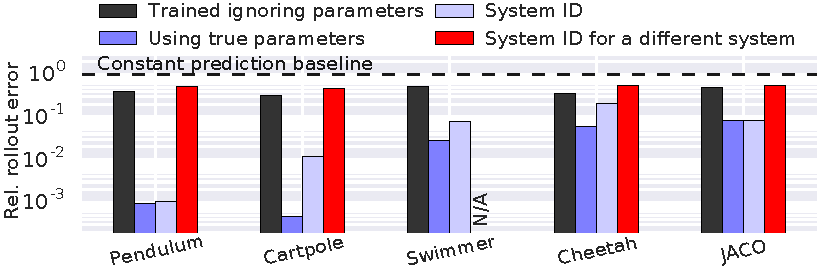
\includegraphics[width=\columnwidth]{figures/quantitative_comparison_rollout_sysid}}
\vspace{-0.1in}
\caption{System identification performance. The y-axis represents 100-step rollout error, relative to the trivial constant prediction baseline (black dashed line). The baseline GN-based model (black bars) with no system identification module performs worst. A model which was always provided the true static parameters (medium blue bars) and thus did not require system identification performed best. A model without explicit access to the true static parameters, but with a system identification module (light blue bars), performed generally well, sometimes very close to the model which observed the true parameters. But when that same model was presented with an ID phase whose hidden parameters were different (but from the same distribution) from its prediction phase (red bars), its performance was similar or worse than the model (black) with no ID information available. (The N/A column is because our Swimmer experiments always varied the number of links as well as parameters, which meant the inferred static graph could not be concatenated with the initial dynamic graph.)}
\label{fig:quantitative_comparison_sysid}
\end{center}
\vskip -0.2in
\end{figure}